\chapter[\texorpdfstring{Дифференцируемость функций комплексного перемен-\protect\linebreak ного. Условия Коши-Римана. Интегральная теорема Коши.}{}]{Дифференцируемость функций комплексного переменного. Условия Коши-Римана. Интегральная теорема Коши.}
\section{Дифференцируемость функций комплексного переменного}

\subsection{Предел. Функции комплексного переменного}
Пусть $\{z_n\}$ -- последовательность чисел из $\bbC$, $z_n=x_n+iy_n, \, n \in \bbN$. 
\begin{defn}
Число $A = a+ib \in \bbC$ называется \textit{пределом последовательности} $\{z_n\}$, если $\forall \epsilon > 0\quad \exists N(\epsilon)$ такое, что $\forall n \ge N(\epsilon) $ справедливо включение $z_n \in B_\epsilon(A) \triangleq \{z_n \;\bigl|\; |z_n-A|<\epsilon \bigl.\}$.
\end{defn}
\begin{defn}
Последовательность $\{z_n\}$ \textit{сходится к бесконечности}, если 
$$
\forall \epsilon > 0\quad \exists N(\epsilon): \fa n \ge N(\epsilon) \quad |z_n|>\epsilon.
$$
\end{defn} 
Это определение эквивалентно тому, что окрестностью бесконечности является внешность круга $\overline{B_\epsilon(0)}$, т.е. множество вида $\overset{\circ} {B}_\epsilon(\infty)\triangleq \{z \;\bigl|\; |z|>\epsilon \bigl.\}$. Обозначим $B_\epsilon(\infty)=\overset{\circ} {B}_\epsilon(\infty) \cup\{\infty\}$.

Пусть $f: G\to \bbC$ - функция, где $G \subset \bboC$. Где ${\bboC =\{\infty\} \cup \{\bbC\}}$ с введенной выше системой окрестностей точки $\infty$. Заметим, что задание комплексной функции $f$ равносильно заданию двух действительных функций $u=u(x,y)$ и $v=v(x,y)$, так как $f(z)=u(x,y)+iv(x,y)$.
\begin{defn}
Точка $z_0 \in \bboC$ называется \textit{внутренней точкой($z_0 \in \interior G$) множества} $G \subset \bboC$, если существует число $\epsilon > 0$ такое, что справедливо включение $B_\epsilon (z_0) \subset G$.
\end{defn} 

\begin{defn}
Точка $z_0 \in \bboC$ называется \textit{предельной точкой множества} $G \subset \bboC$, если для любого числа $\epsilon > 0$ в проколотой окрестности $\overset{\circ} {B}_\epsilon(z_0)\triangleq \{z \;\bigl|\; 0<|z-z_0|<\epsilon \bigl.\}$ имеется по крайней мере одна точка (а потому и бесконечно много точек) из $G$ (т.е. $\overset{\circ} {B}_\epsilon(z_0) \cap G \neq \emptyset,\; \forall\epsilon > 0$).
\end{defn}

\begin{defn}
Пусть $f: G\subset \bboC \to \bboC$ -- функция и точка $z_0$ -- предельная точка для $G$. Тогда число $A \in \bboC$ называется \textit{пределом функции в точке $z_0$ по множеству $G$}, если 
$$
\forall \epsilon > 0 \ex \delta = \delta(\epsilon)>0:\fa z \in \overset{\circ} {B}_\delta(z_0)\cap G \quad f(z) \in B_\epsilon(A). 
$$ 
\end{defn}

\begin{thm} [о трех функциях]
\label{exp14}
Пусть $z_0$ -- предельная точка множества $D\subset \bbC$. Пусть $D = D_f=D_g=D_h$ и $\exists \delta > 0$ $\forall z \in D \cap \dneio{\delta}{z_0}:$
$$f(z)\le g(z) \le h(z),$$ тогда если $\exists \lim_{z \to z_0}\limits f(z) = A \in \bbC$ , $\exists \lim_{z \to z_0}\limits h(z) = A$, тогда и $\exists \lim_{z \to z_0}\limits g(z) = A$.
\end{thm}

\subsection{Дифференцирование функций комплексного переменного}
\begin{defn}
\label{exp5}
Если функция  $f : B_r(z_0) \to \bbC $ такова, что существует конечный предел отношения
$$
\frac{f(z)-f(z_0)}{z-z_0} \quad\text{при}\quad z \to z_0,
$$
то этот предел называется \textit{производной функции} $f$ в точке $z_0$ и обозначается $f'(z_0)$. 
\end{defn}
Пусть $\Delta z = z - z_0$ и $\Delta f = f(z) - f(z_0)$. Определение \ref{exp5} означает, что $\forall \epsilon > 0 \ex \delta=\delta(\epsilon)>0$ такое, что для $\forall \Delta z:\quad 0 <|\Delta z| <\delta$ справедливо 
\begin{equation}
\label{exp7}
\left|\frac{\Delta f}{\Delta z} - f'(z_0) \right| < \epsilon.
\end{equation}
Отсюда следует, что 
\begin{equation}
\label{exp6}
\Delta f = f'(z_0)\Delta z + \alpha(\Delta z),
\end{equation}
где функция $\alpha(\Delta z)$, определяемая из равенства \eqref{exp6} в силу \eqref{exp7} удовлетворяет условию $\lim_{\Delta z \to 0}\limits \frac{\alpha(\Delta z)}{\Delta z} = 0$. (такая функция называется $o-$малой и обозначается $o(\Delta z)$.

\begin{defn}
Функция $f : B_r(z_0) \to \bbC $ дифференцируема в точке $z_0 \in \bbC$, если справедливо представление 
\begin{equation}
\label{exp4}
\Delta f = A\cdot \Delta z + \alpha(\Delta z), \fa \Delta z: 0 < |\Delta z|< r,
\end{equation}
где А не зависит от $\Delta z$, а функция $\alpha(\Delta z)$ является $o(\Delta z)$.
\end{defn}

\begin{lemm}
Функция $f : B_r(z_0) \to \bbC $ дифференцируема в точке $z_0$ $\Longleftrightarrow$ существует производная $f'(z_0)$, причем в формуле \eqref{exp4} число $A=f'(z_0)$.
\end{lemm}

\section{Условия Коши-Римана}  
Пусть $f(z)=u(x,y)+iv(x,y)$, где $z=x+iy$, $z_0=x_0+iy_0$; $\Delta z=z-z_0$, или $\Delta z = \Delta x + i\Delta y$, где $\Delta x = x-x_0$ и $\Delta y =y-y_0$; $\Delta f = \Delta u + i\Delta v$, где $\Delta u = u(x,y)-u(x_0,y_0)$,  $\Delta v = v(x,y)-v(x_0,y_0)$. 
\begin{thm} [Условия Коши-Римана]
Для того, чтобы функция $f: G  \to \bbC,\, G \subset \bbC$ была дифференцируема в точке $z_0\in \interior G$, необходимо и достаточно, чтобы
\begin{enumerate}
\item
Функции $u(x,y)$ и $v(x,y)$ были дифференцируемы в точке $(x_0,y_0) \in \bbR^2$ (как функции двух действительных переменных $x$ и $y$).
\item
В точке  $(x_0,y_0)$ были выполнены следующие условия (называемые условиями Коши-Римана) \footnote{Для краткости, примем следующее обозначение для частных производных $\pd{\textstyle u}{ \textstyle x}=u'_x.$}:
\begin{equation}
\label{exp17}
\begin{split}
&u'_x(x_0,y_0) = v'_y(x_0,y_0), \\ &u'_y(x_0,y_0) = -v'_x(x_0,y_0).
\end{split}
\end{equation}
При этом
\begin{equation}
\label{exp8}
f'(z_0) = u'_x(x_0,y_0) + iv'_x(x_0,y_0)= u'_y(x_0,y_0) -iv'_y(x_0,y_0).
\end{equation}
\end{enumerate}
\end{thm}
\begin{proof}
$ $\linebreak
\vspace*{-\baselineskip}
\begin{itemize}
\item[$\Longrightarrow$:]
Пусть $\exists f'(z_0) = a+ib $. Тогда $\Delta f = f'(z_0)\Delta z + \alpha(\Delta z)$, где $\frac{\alpha(\Delta z)}{\Delta z}\xrightarrow{\Delta z \to 0}0$. Но, с другой стороны, $\Delta f = \Delta u + i \Delta v$. А значит
$$
\Delta u + i \Delta v = \underbrace{(a+ib)}_{f'(z_0)}(\Delta x + i \Delta y) + \underbrace{\alpha_1(\Delta x, \Delta y) +i \alpha_2(\Delta x, \Delta y)}_{\alpha(\Delta z)}
$$
Приравниваем действительные и мнимые части слева и справа:
\begin{equation}
\label{exp15}
\begin{cases}
\Delta u = a\Delta x - b \Delta y + \alpha_1(\Delta x, \Delta y) \\
\Delta v = b\Delta x + a \Delta y + \alpha_2(\Delta x, \Delta y).
\end{cases}
\end{equation}
Рассмотрим $0 \le |\alpha_1(\Delta x, \Delta y)| \le |\alpha(\Delta z)|$ (катет не длиннее гипотенузы, $|\alpha|^2=|\alpha_1|^2 + |\alpha_2|^2 $). Тогда
$$
\underbrace{{{\vphantom{\frac{0}{0}}}}0}_{=0} \le \frac{|\alpha_1(\Delta x, \Delta y)|}{|\Delta z|} \le \underbrace{\frac{|\alpha(\Delta z)|}{|\Delta z|}}_{\xrightarrow{\Delta z \to 0} 0 }.
$$
Из теоремы \hyperref[exp14]{о трех функциях} следует: $\exists \lim_{\substack{\Delta x \to 0\\ \Delta y \to 0}}\limits \frac{|\alpha_1(\Delta x,\Delta y)|}{\sqrt{\Delta x ^2 + \Delta y^2}} = 0.$
Аналогично, $\exists \lim_{\substack{\Delta x \to 0\\ \Delta y \to 0}}\limits \frac{|\alpha_2(\Delta x,\Delta y)|}{\sqrt{\Delta x^2 + \Delta y^2}} = 0$. 
Отсюда и из равенства \eqref{exp15} следует дифференцируемость функций $u(x,y)$ и $v(x,y)$ в точке $(x_0,y_0) \in \bbR^2$, причем 
\begin{equation}
\label{exp16}
\begin{split}
&u'_x(x_0,y_0) = a, \qquad u'_y(x_0,y_0) = -b,\\
&v'_y(x_0,y_0) = b, \qquad v'_x(x_0,y_0) = a.
\end{split}
\end{equation}

Используя равенства \eqref{exp16} убеждаемся, что выполнены условия Коши-Римана \eqref{exp17}, причем 
$$
f'(z_0) = a+ib = u'_x(x_0,y_0) + iv'_x(x_0,y_0)= u'_y(x_0,y_0) -iv'_y(x_0,y_0)
$$ 
\item[$\Longleftarrow$:]
Пусть функции $u(x,y)$, $v(x,y)$ дифференцируемы в точке $(x_0,y_0)$, выполнены условия Коши-Римана \eqref{exp17}. Тогда в точке $z_0=x_0+iy_0$
\begin{multline*}
\Delta f = \Delta u + i\Delta v \xlongequal{u,v\;\text{\scriptsize дифф.}} u'_x\Delta x + \overbrace{u'_y}^{-v'_x}\Delta y + \alpha_1(\Delta x,\Delta y)+ \\+ i\bigr(v'_x\Delta x + \overbrace{v'_y}^{u'_x}\Delta y + \alpha_2(\Delta x,\Delta y)\bigl) \myeq{\eqref{exp17}}\\\myeq{\eqref{exp17}} (u'_x+iv'_x)(\Delta x + i \Delta y) + \alpha_1(\Delta x,\Delta y)+ i\alpha_2(\Delta x,\Delta y) = A\cdot\Delta z + \alpha(\Delta z),
\end{multline*}
где число $A = u'_x(x_0,y_0)+iv'_x(x_0,y_0)$, функция $\alpha = \alpha_1+\alpha_2$, причем, поскольку  $\exists \lim_{\substack{\Delta x \to 0\\ \Delta y \to 0}}\limits \frac{|\alpha_1(\Delta x,\Delta y)|}{\sqrt{(\Delta x)^2 + (\Delta y)^2}} = 0$, $\exists \lim_{\substack{\Delta x \to 0\\ \Delta y \to 0}}\limits \frac{|\alpha_2(\Delta x,\Delta y)|}{\sqrt{(\Delta x)^2 + (\Delta y)^2}} = 0$, то

$$
\left| \frac{\alpha(\Delta z)}{\Delta z} \right| \le \frac{|\alpha_1(\Delta x,\Delta y)|}{\sqrt{(\Delta x)^2 + (\Delta y)^2}} + \frac{|\alpha_2(\Delta x,\Delta y)|}{\sqrt{(\Delta x)^2 + (\Delta y)^2}} \xrightarrow{(\Delta x,\Delta y) \to (0,0)} 0,
$$
т.е. функия $f$ дифференцируема в точке $z_0$, и верна формула \eqref{exp8}.
\end{itemize}
Теорема доказана.
\end{proof}


\section{Интегральная теорема Коши}
\subsection{Регулярные функции}
Аналогично $\bbR^2$ мы назовем множество $G$ из $\bbC$ (или $\bboC$):
\begin{itemize}
\item
\textit{открытым}, если для любой его точки $z_0$ найдется ее окрестность $B(z_0)$, принадлежащая этому множеству;
\item
\textit{замкнутым}, если оно содержит все свои предельные точки;
\item 
\textit{областью}, если множество обладает следующими двумя свойствами:
\begin{enumerate}
\item 
для любой точки $z_0 \in G$ существует окрестность этой точки, принадлежащая $G$ (\textit{открытость});
\item 
для любых двух точек $z_1,z_2 \in G$ существует лежащий в $G$ путь с концами $z_1$ и $z_2$ (\textit{линейная связность});
\end{enumerate}
\item
\textit{односвязной областью}, если любой простой замкнутый контур, целиком лежащий в ней, может быть непрерывной деформацией стянут в точку, постоянно оставаясь внутри области. 
\end{itemize}

\begin{defn}
Пусть $G$ -- область в $\bbC$. Функция $f: G \to \bbC$ называется \textit{регулярной в области G}, если она дифференцируема на $G$ и ее производная $f' : G \to \bbC$ является непрерывной функцией. Говорят, что $f : G \to \bbC$ \textit{регулярна в mочке} $z_0 \in G$, если она регулярна в некоторой окрестности этой точки. 
\end{defn}


\subsection{Интегрирование функции комплексного переменного}
\begin{defn}
\textit{Непрерывной кривой} называется геометрическое место точек $z$ комплексной плоскости $\bbC$, удовлетворяющих некоторому параметрическому уравнению $z=z(t) = x(t) + iy(t)$, где $x(t)$ и $y(t)$ -- непрерывные функции действительного переменного $t$ на отрезке $[t_0,t_1]$. Непрерывная кривая~--- \textit{простая}, если $\forall t',t'' \in [t_0,t_1]: t'\ne t'' \Rightarrow z(t') \ne z(t'')  $, кроме, возможно $z(t_0) = z(t_1)$ . Непрерывная кривая --- \textit{замкнутая}, если  $z(t_0) = z(t_1)$ 
\end{defn}

При изменении параметра $t$ на отрезке $[t_0 , t_1$] в одном направлении (от $t_0$ к $t_1$ или наоборот) точка $z(t)$ совершает обход кривой $\gamma$. Выбор направления обхода кривой $\gamma$ называется ориентацией кривой, а кривая с выбранной ориентацией называется \textit{ориентированной кривой} или \textit{контуром}.

Скажем, что на кривой $\gamma$ выбрана \textit{ориентация, индуцированная данной параметризацией} $z(t)$, $t \in[t_0 , t_1]$, если на кривой выбрано направление движения, соответствующее возрастанию $t$. 

\begin{defn}
Непрерывная кривая $\gamma \subset \bbC$ называется \textit{гладкой}, если она допускает параметрическое представление с помощью комплекснозначной функции действительного аргумента $z = z(t) = x(t) + iy(t)$, $t \in [t_0 , t_1]$, у которой функции $x(t)$ и $y(t)$ непрерывны, имеют непрерывные производные $x'(t)$ и $y'(t)$ и $z'(t) = x'(t) +iy'(t) \ne 0$ всюду на отрезке $[t_0 , t_1]$, причем если кривая замкнута, то $z'(t_0 +0)= z'(t_1 - 0)$.
\end{defn}

\begin{defn}
Пусть дан непрерывный контур $\gamma$ в $\bbC$ с параметризацией $z =z(t)$. Пусть существует конечное разбиение $\{\theta_k\}^m_{k=0}$ отрезка $[t_0 , t_1]$, т.е. $t_0 = \theta_0 < \theta_1 < ... < \theta_m = t_1$ такое, что контуры $\gamma_k$, определяемые функциями $z = z(t)$, $t \in [\theta_{k-1}, \theta_k]$, являются гладкими контурами с той же, что и у контура $\gamma$, ориентацией. Тогда контур $\gamma$ называется \textit{кусочном-гладким контуром}, или \textit{объединением гладких контуров } $\{\gamma_k\}$, т.е. $\gamma = \gamma_1 \cup \gamma_2 \cup\dots \cup\gamma_m$. 
\end{defn}


  \mywrappict{pictures/ch33pict1}{0.25}
Пусть дан кусочно-гладкий контур $\gamma$ с параметризацией $z=z(t)$, $t \in[t_0 , t_1]$, где $z(t_0)$ -- начало, а $z(t_1)$ -- конец контура $\gamma$. 

Пусть выбрано конечное \textit{разбиение отрезка} $[t_0, t_1]$ вида
\begin{equation}
\label{exp19}
\lambda \triangleq \{\tau_k\; \bigr|\bigl.\; k \in \overline{1,m_\lambda},\; t_0=\tau_0 < \tau_1 < \tau_2 < \dots < \tau_{m_\lambda} = t_1 \}.
\end{equation}
\textit{Мелкостъю разбиения} $\lambda$ назовем величину
$$
|\lambda| = \max \{\tau_k - \tau_{k-1} \; \bigr|\bigl.\; k \in \overline{1,m_\lambda}\}.
$$
Пусть при каждом $k \in \overline{1,m_\lambda}$, произвольно выбрана точка

\begin{equation}
\label{exp23}
\zeta_k \in \{z(t)\; \bigr|\bigl.\; t \in [\tau_{k-1},\tau_k]\},
\end{equation}
т.е. точка $\zeta_k$ принадлежит дуге $\stackrel{\smile}{z_{k-1}, z_k} \subset \gamma$, где $z_k \triangleq z(\tau_k)$.

\begin{defn}
\label{omg}
Пусть дана непрерывная на кусочно-гладком контуре $\gamma$ функция $w=f(z)$. Определим выражение
\begin{equation}
\label{exp18}
\sigma(\lambda) \triangleq \sum\limits_{k=1}^{m_{\lambda}} f(\zeta_k)\Delta z_k, \quad\text{где}\quad \Delta z_k \triangleq z_k - z_{k-1},
\end{equation}
которое будем называть \textit{интегральной суммой функции} $f$, соответствующей разбиению $\lambda$.
\end{defn}

Если существует конечный предел интегральных сумм \eqref{exp18} при $|\lambda| \to 0$, не зависящий от выбора разбиения $\lambda$ \eqref{exp19} и точек $\{\zeta_k\}$ \eqref{exp23}, то этот предел называется интегралом от функции $f$ по контуру $\gamma$, который обозначается

\begin{equation}
\label{exp22}
\int_\gamma f(z)\,dz.
\end{equation}

\begin{thm}
\label{exp21}
Пусть дана непрерывная на кусочно-гладком контуре $\gamma$ функция $f(z)$. Тогда интеграл \eqref{exp22} существует и справедлива формула
\begin{equation}
\label{exp24}
\int _\gamma f(z) \,dz = \int _\gamma(u(x,y)\,dx - v(x,y)\,dy)+i\int_\gamma (v(x,y)\,dx +u(x,y)\,dy),
\end{equation}
где $f(z) = u(x, y)+ iv(x, y$), и стоящие справа в формуле \eqref{exp24} два интеграла являются криволинейными интегралами второго рода от действительных функций действительных переменных по контуру $\gamma$ на евклидовой плоскости $\bbR^2$.
\end{thm}


\begin{cons}
Пусть дана непрерывная на кусочно-гладком контуре $\gamma$ функция $f(z)$. Тогда справедлива формула 
\begin{equation}
\label{abc1}
\int _\gamma f(z) \,dz = \int _{t_0}^{t_1} f(z(t))\cdot z'(t) \,dt,
\end{equation}
где в \eqref{abc1} интеграл в правой части от комплексной функции действительного переменного определяется по формуле
\begin{equation}
\label{kek2}
\int _{t_0}^{t_1}(u(t)+iv(t)) \,dt \triangleq \int _{t_0}^{t_1}u(t) \,dt + i \int _{t_0}^{t_1}v(t) \,dt.
\end{equation}
\end{cons}

\subsection{Интегральная теорема Коши}
\addmppict{pictures/ch33pict2}{0.2}{
\begin{thm}[Коши]
\label{abc2}
Для всякой регулярной функции $f:G\to\bbC$, заданной в односвязной области G, справедливо равенство
\begin{equation}
\label{abc3}
\int_\gamma f(z)\,dz = 0.
\end{equation}

\parshape 2 
0pt \dimexpr\textwidth\relax
0pt \dimexpr(\textwidth)\relax
где интеграл берется по любому замкнутому простому кусочно-гладкому контуру $\gamma$, лежащему в области $G$.
\end{thm}
}
\begin{proof}
Для заданного в теореме контура $\gamma$ запишем формулу \eqref{exp24}:
\begin{equation}
\label{abc4}
\int_\gamma f(z)\,dz = \int_\gamma (u+iv)\,(dx+idy) = \underbrace{\int _\gamma(u\,dx - v\,dy)}_{\textstyle\triangleq J_1} + i\cdot\underbrace{\int_\gamma (v\,dx +u\,dy)}_{\textstyle\triangleq J_2},
\end{equation}

Через $D$ обозначим односвязную область в $G$, границей которой является данный контур $\gamma$. Нам известна следующая формула Грина:
\begin{equation}
\label{abc6}
\int_\gamma P\, dx + Q\, dy = \iint_D \left(\pd{Q}{x}-\pd{P}{y}\right)\,dx\,dy ,
\end{equation}
где $P(x, y)$ и $Q(x, y)$ - действительные функции переменных $x$, $y$, непрерывные со своими частными производными первого порядка в
замкнутой области $\overline{D} = D \cup \gamma$. 

В силу непрерывной дифференцируемости функций $u$ и $v$ на односвязной области $G$, следующей из регулярности функции $f$, формула Грина \eqref{abc6} и \hyperref[exp17]{условия Коши-Римана} дают для интегралов \eqref{abc4}
\begin{equation*}
\begin{split}
&J_1 \myeq{\eqref{abc6}} \iint_D \left(-\pd{v}{x}-\pd{u}{y}\right)\,dx\,dy \xlongequal{\text{\scriptsize УКР}} 0,\\
&J_2 \myeq{\eqref{abc6}} \iint_D \left(\pd{u}{x}-\pd{v}{y}\right)\,dx\,dy \xlongequal{\text{\scriptsize УКР}} 0,
\end{split}
\end{equation*} 
т.е. равенство \eqref{abc3} доказано, а значит теорема доказана.
\end{proof}
%\addmppict[0.8]{pictures/ch33pict3}{0.4}{
\usepict[0.2]{ch33pict3}
\begin{defn} \label{ch33defn1}
\textit{Областью с кусочно-гладкой границей} будем называть область $G \subset \bboC$, граница $\partial G=\Gamma$ которой является объединением конечного числа гладких ограниченных кривых $\Gamma_1 , \dots , \Gamma_m$, любые две из которых могут иметь общими лишь концевые точки. 

Эти кривые $\Gamma_1 , \dots , \Gamma_m$ будем называть гладкими компонентами границы $\Gamma$ области $G$. Эти компоненты бывают двух типов:
\end{defn}
%}

\begin{enumerate}
\item
Кривая $\Gamma_k$ --- \textit{правильной гладкой компонентой} $\Gamma$, если в каждой окрестности каждой точки $z_0 \in \;\buildrel\circ\over\Gamma_k$ ($\buildrel\circ\over\Gamma_k$ --- кривая $\Gamma_k$ без концевых точек) находятся как точки из области $G$, так и из $\bbC \setminus G\cup\Gamma$. 

\item
Кривая $\Gamma_k$ --- \textit{разрезом}, если для каждой точки $z_0 \in\; \buildrel\circ\over\Gamma_k$ существует окрестность $B_\epsilon(z_0)$ такая, что $B_\epsilon(z_0)\setminus\Gamma_k \subset G$.
\end{enumerate}
\begin{defn} \label{ch33defn2} 
Будем считать, что кусочно-гладкая граница $(\partial G)^{+}$ \textit{положительно ориентирована относительно области $G$}, если при обходе $(\partial G)^{+}$ область $G$ остается слева (при этом считается, что разрез проходится дважды: в одну сторону, потом в противоположную). Аналогично, определим отрицательно ориентрированную границу относительно области $G$, которую обозначим $(\partial G)^{-}.$
\end{defn}

Если $f:\overline{G}\to\bbC$ будем продолжать по непрерывности на $\partial G$, то не исключаем, что на разрезы $f$ может продолжаться по-разному, т.е. пределы с разных берегов разреза могут отличаться. 

\begin{thm}[интегральная теорема Коши для односвязных областей]\label{abcd1}
Пусть дана ограниченная односвязная область $G$ с кусочно-гладкой положительно ориентированной границей $\Gamma$. Пусть функция $f:\overline{G}\to\bbC$ регулярна на области $G$ и непрерывна на замыкании области $\overline{G}=G\cup\Gamma$. Тогда
\begin{equation}
\label{abc10}
\int_{\Gamma} f(z)\,dz = 0.
\end{equation}
\end{thm}
\begin{proof}
Приведем доказательство этой теоремы для случая, когда добавлением к границе $\Gamma$ конечного числа разрезов оставшиеся точки области $G$ можно представить в виде объединения конечного числа звездных множеств. 
\begin{defn}
\label{abc8}
Ограниченная область $G$ называется \textit{звездным множеством}, если граница $\Gamma$ области $G$ может быть задана в виде
\begin{equation}
\label{abc5}
\Gamma = \{ z \bigr|\bigl. z = z_0+z_1(t),  \alpha \le t \le \beta, z_1(\alpha) = z_1 (\beta) \},
\end{equation} 
где $z_0 \in G$ называется \textit{центром звездного множества}, $z_1 :[\alpha, \beta] \to \bbC$ --- кусочно-гладкая функция, причем должны выполняться включения
\begin{equation}
\label{abc7}
\Gamma_\lambda \triangleq \{ z \bigr|\bigl. z = z_0+\lambda z_1(t),  \alpha \le t \le \beta\} \subset G, \fa \lambda \in [0,1).
\end{equation}

Проще говоря, множество $G$ называется \textit{звездным}, если можно найти такую точку (\textit{центр зведного множества}), что все прямые отрезки, соединяющие ее с любой другой, целиком принадлежат $G$.
\end{defn}
\begin{center}
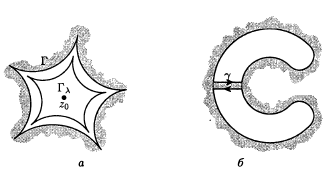
\includegraphics[width=0.7\textwidth]{pictures/ch33pict4}\refstepcounter{pictnumber} Рис. \thepictnumber
\end{center}

Доказательство достаточно провести для случая, когда $G$ есть звездное множество с центром в точке $z_0 = 0$. Покажем это. 

Допустим, что его центр $z_0 \ne 0$. Сделав  замену $\tilde z = z - z_0$ , $\tilde \Gamma = \Gamma - z_0$, $\tilde{G} = G - z_0$, получим звездное множество $G$ с центром в точке $0$, причем
$$
\int_{\Gamma} f(z)\,dz = \int_{\tilde \Gamma} f(\tilde z +z_0)\,d\tilde z = \int_{\partial\tilde G} \tilde f(\tilde z)\,d\tilde z ,
$$
где $\tilde f(\tilde z) = f(\tilde z + z_0 )$ есть регулярная функция, и если покажем, что последний интеграл равен нулю, то и исходный равен нулю.

Итак, считаем, что центр множества $G$ есть точка $z_0 =0$. Тогда
кривая $\Gamma_\lambda$ из \eqref{abc7} принимает вид:
$$
\Gamma_\lambda \triangleq \{ z \bigr|\bigl. z = \lambda z_1(t), \alpha \le t \le \beta\},\quad\lambda \in (0,1).
$$
Так как по определению \ref{abc8} звездного множества справедливы включения $\Gamma_\lambda \subset G$, то по теореме Коши \ref{abc2}  справедливо равенство
\begin{equation}
\label{abc11}
\int_{\Gamma_\lambda} f(\zeta)\,d\zeta = 0.\quad \forall \lambda \in (0,1).
\end{equation}
Для каждого $\lambda \in (0,1)$ делаем замену переменного $\zeta = \lambda z$. Тогда $\zeta \in \Gamma_\lambda \Leftrightarrow z \in \Gamma$. В силу этой замены равенство \eqref{abc11}  принимает вид
\begin{equation}
\label{abc9}
\int_{\Gamma} f(\lambda z)\lambda\,dz = 0, \; \text{откуда} \; \int_{\Gamma} f(\lambda z)\,dz = 0, \fa \lambda \in (0,1)
\end{equation}

Так как функция $f$ непрерывна на ограниченном замкнутом множестве $\overline{G}$, то она равномерно непрерывна на $\overline{G}$. Это значит, что $\forall \epsilon > 0 \ex \delta = \delta (\epsilon) > 0, \forall z',z'' \in \overline{G}, |z'-z''|<\delta \Rightarrow |f(z')-f(z'')| < \epsilon$.  Поэтому $\forall z \in \Gamma$ получаем $|z-\lambda z|=(1-\lambda)|z| \le (1-\lambda)C_0$, где $C_0=\max\{|z|\bigr|\bigl. z\in \Gamma\}$.

Выбрав $\lambda_\epsilon \in (0, 1)$, удовлетворяющее неравенству $(1 - \lambda_\epsilon) < \delta(\epsilon)/C_0 $, получаем $|z - \lambda_\epsilon z| < \delta(\epsilon),\, \forall z \in \Gamma$. Поэтому из \eqref{abc9} следует:
\begin{multline}
\left|\int_{\Gamma} f(z) \,dz \right| = \left|\int_{\Gamma} f(z) \,dz - 0 \right| = \left|\int_{\Gamma} (f(z) - f(\lambda_\epsilon z))\,dz \right| \le \\
\le \int_{\Gamma} |f(z) - f(\lambda_\epsilon z)|\,|dz| \le \epsilon \int_{\Gamma} |dz|.
\end{multline}
В силу произвольности числа $\epsilon > 0$ получаем равенство \eqref{abc10}.

\noindent 
Теорема доказана.
\end{proof}

\begin{thm}[обобщенная интегральная теорема Коши]\label{abc28}
Пусть дана ограниченная область $G$ с кусочно-гладкой положительно ориентированной границей $\Gamma$. Пусть функция $f:\overline{G}\to\bbC$ регулярна на области $G$ и непрерывна на замыкании области $\overline{G}=G\cup\Gamma$. Тогда
\begin{equation}
\int_{\Gamma} f(z)\,dz = 0.
\end{equation}
\end{thm}
\usepict{ch33pict5}
\begin{proof}
Поскольку область ограничена, то значит одна группа компонент, <<внешняя>> компонента, образует кусочно-гладкий замкнутый контур, который отделяет $G$ от бесконечности. (см. рис. \ref{ch33pict5})

Добавим к каждой <<внутренней>> компоненте границы $\partial G$ дополнительный разрез, соединяющий его с <<внешней>> компонентой. 
Итак, мы конечным числом дополнительных непересекающихся между собой разрезов $R_1,\dots R_p$ разбили область $G$ на  подмножества $G_1,\dots, G_m$. Эти подмножества, по построению,являются ограниченными односвязными областями с кусочно-гладкими границами. Тогда по интегральной теореме Коши для односвязных множеств:
$$
\underbrace{0=\sum_{j=1}^m \int_{(\partial G_j)^+} f(z) \,dz }_{\text{\scriptsizeт.к. каждый интеграл} =0} = \int_{(\partial G)^+} f(z)\,dz + \sum_{k=1}^{m} \underbrace{\left( \int_{(R_k)^+}f(z)\,dz + \int_{(R_k)^-}f(z)\,dz \right)}_{\textstyle =0 \fa s}
$$ 
Отсюда
$$
\int_{(\partial G)^+} f(z)\,dz = 0.
$$
\noindent 
Теорема доказана.\footnote{Хочу обратить ваше внимание, что мы везде писали $\Gamma$ (следуя обозначениям Е.С.~Половинкина), однако подразумевали, что берем положительно ориентированную границу $G$ относительно области $G$. Т.е. нагляднее было бы писать $(\partial G)^{+}$. Просто не забывайте, что в Теоремах \ref{abcd1} и \ref{abc28}  нужна положительно ориентированная граница. }
\end{proof}